\chapter{Related Works}

\section{Haptic Survey and PA Model}
In the past literature or survey related to haptics, various kinds of haptic devices and their characteristics are extensively mentioned. However, each classification is different. A detailed report on haptics\cite{ref_S001} pointed out two critical factors for judging and measuring haptic devices: \textbf{Physicality} whether the physicality of the haptic device is consistent with the target object, and \textbf{Actuation} whether the device relies on servo drive to achieve haptic effects. 

\begin{figure}[h]
\centering
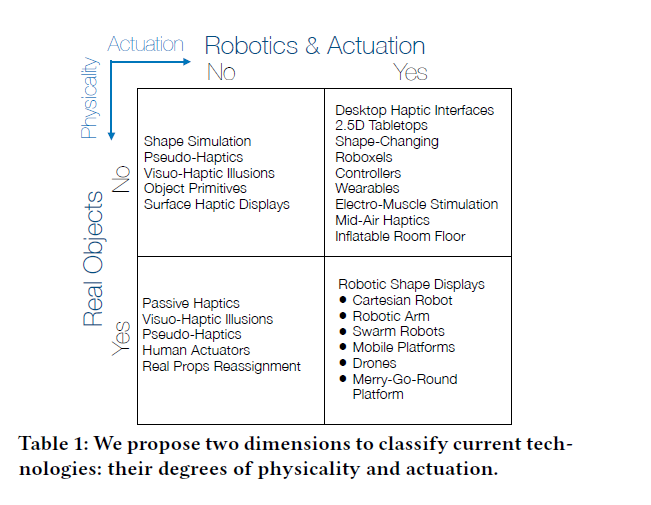
\includegraphics[width=0.8\textwidth]{A_thesis/figures/001.png}
\caption{PA Model}
\end{figure}


Based on these two features, all haptic technologies are divided into four parts. For instance, haptic technologies involving shape simulation firstly do not have devices physically inconsistent with the target object. And since it's based on the theory of force visual simulation, there are no servos or motors used in the entire device, thus falling into the first quadrant (NN). Haptic technology widely used for achieving goals through robotics, such as using a robotic arm to achieve the haptic simulation effect of virtual space objects, is classified in the fourth quadrant (YY) because both physicality and actuation are the same as the target object. As for single-performance focus, for example, in the third quadrant, haptic technology shows the same physical properties as the target object, but does not use driving technology. Techniques such as pseudo-touch and visual-touch technology mostly show different effects based on changing visual parameters (lighting, texture) or tracker display effects (Optitrack, HTC trackers).

\begin{figure}[h]
\centering
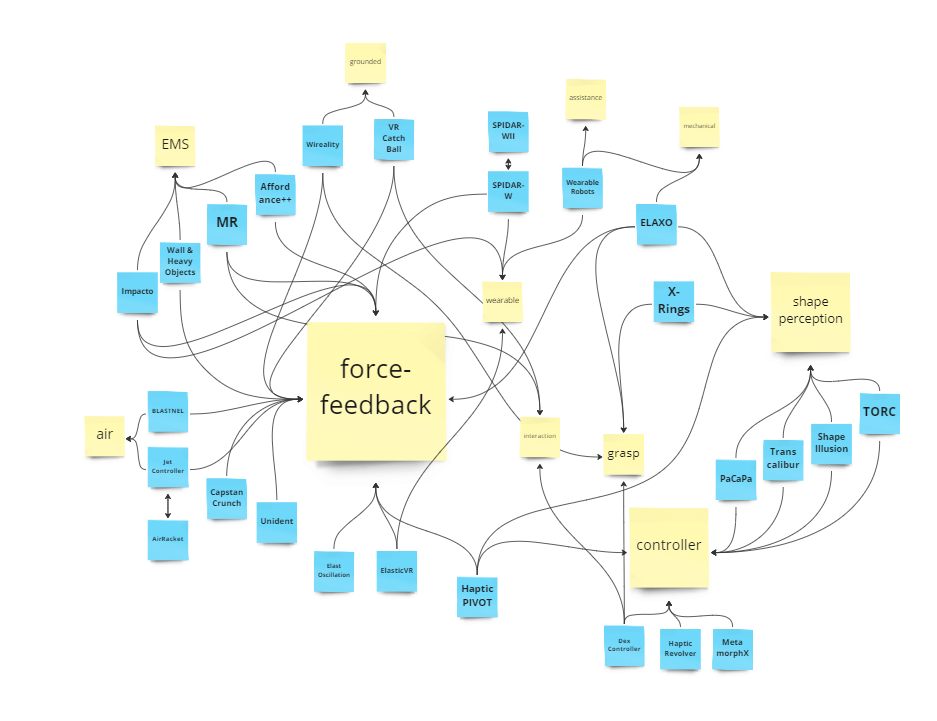
\includegraphics[width=0.8\textwidth]{A_thesis/figures/002.png}
\caption{Rearrangement of multiple references}
\end{figure}


\section{Research Objectives}
Although the PA model theory mentioned above can be used to categorize haptic technology, the initial consideration of this research theme is more inclined to the feasibility of using some robot technology for implementation cost. However, the research purpose will not be the same physical effect as in reality. Therefore, although the PA model has supplemented theoretical knowledge, it does not have a significant effect on its research analysis. After referring to the PA model, according to the research objectives of haptics, the related haptic technologies are divided into the following four areas: object properties reproduction, user Action Assistance, mechanical process performance, and innovative interaction methods. The logic for judgment is as follows:
\begin{enumerate}
    \item Whether there are already existing interaction patterns in reality ?
    \item Whether it is necessary to display haptic effects with multiple different virtual items ?
    \item Whether the user's actions in the usage scenario are dynamic ?
\end{enumerate}

\begin{figure}[h]
\centering
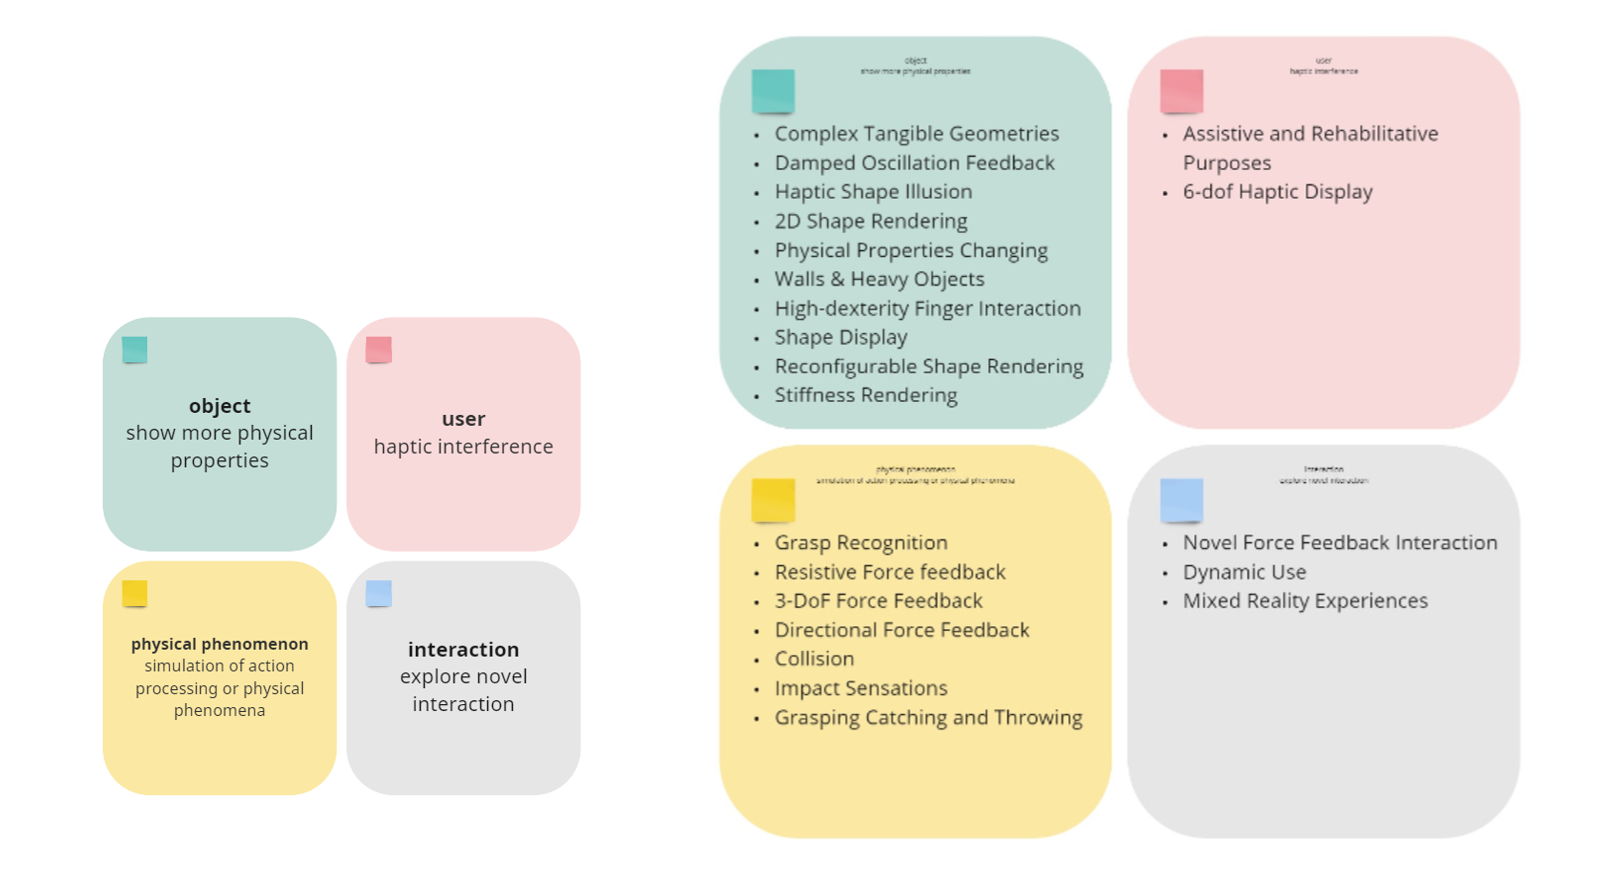
\includegraphics[width=0.8\textwidth]{A_thesis/figures/003.png}
\caption{Classification by research objective}
\end{figure}

\subsection{Object Properties Reproduction}
Haptic devices in this category mainly target virtual objects, aiming to generate or change new object properties. For example, using a cable to fix the user's hand and body to maintain a certain range to make users can feel the outline of complex polygons\cite{ref_003}. By using rubber bands and heavy components to simulate the damped oscillation\cite{ref_006}, it has a noticeable force feedback effect on floating objects and container objects. Using shape illusion to change haptic perception information to simulate virtual objects that do not entirely match the actual shape\cite{ref_012}. Using deformable haptic devices to actually represent handheld items in virtual space\cite{ref_013}. By adjusting the variable torque of CMG devices to show different physical properties such as inertia and viscosity of different objects\cite{ref_017}. By limiting muscles with EMS devices to show heavy objects or walls with large mass\cite{ref_EMS003}. Using the rotation of the wheel to show the texture and roughness on the desktop\cite{ref_MR001}. Miniature devices show the hardness of objects by outputting object resistance\cite{ref_MR004}. By changing the shape of the device to simulate virtual objects of different sizes\cite{ref_MR005}.

\begin{figure}[h]
\centering
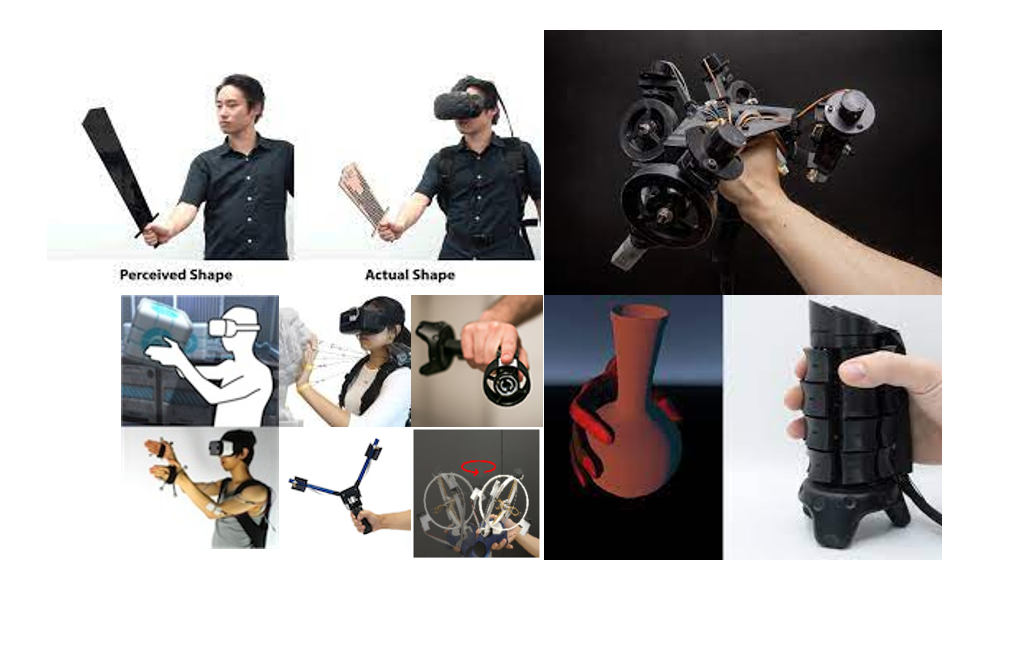
\includegraphics[width=0.8\textwidth]{A_thesis/figures/007.png}
\caption{Research cases of object group}
\end{figure}

\subsection{User Action Assistance}
Corresponding to objects is the impact that mechanical devices have on users themselves. Note that no virtual items are involved in the use and operation of these devices, that is, there are no items as interaction mediums and objects in this type of scenario. These mechanical devices serve not only as action support for users in virtual space but also as auxiliary devices for daily exercise. For example, using hand exoskeletons can enhance user movement in virtual environments and also serve as auxiliary devices for rehabilitation training\cite{ref_002}. Using multiple actuators and fixed devices has achieved the effect of mechanical hints for user positions and movements in virtual space\cite{ref_010}.

\begin{figure}[h]
\centering
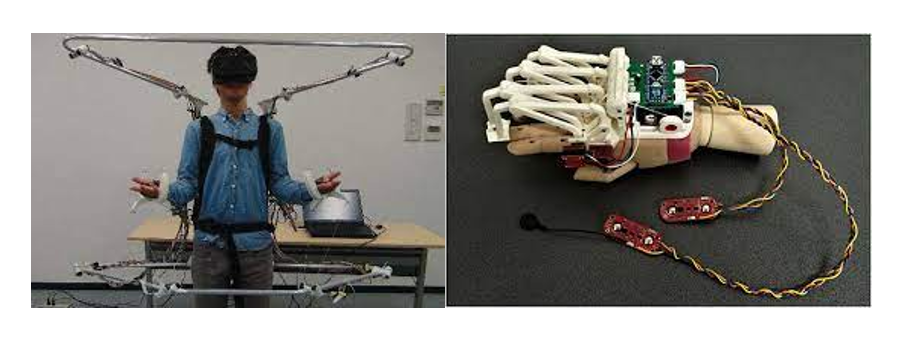
\includegraphics[width=0.75\textwidth]{A_thesis/figures/008.png}
\caption{Research cases of user group}
\end{figure}

\subsection{Mechanical Force Generation}
In addition to focusing on object attributes and user actions, a group of researches pay more attention to the implementation of "force". Force in its basic definition is the result of interactions between two objects. Conceptually representative examples include impact force simulation widely cited using EMS and electromagnets\cite{ref_MR001}. Beyond the usual resistance, by using air propulsion jets to achieve haptic feedback\cite{ref_007}. Also using air propulsion completed directional haptic feedback to enhance the virtual racket sports experiences\cite{ref_008}. As well as compressed air providing full body impact and collision force feedback\cite{ref_015}. Different from contact resistance, continuous resistance has been achieved through rubber\cite{ref_005}. Also, the change of centrifugal force is used to describe the user's grabbing and throwing actions\cite{ref_MR003}. And some of researchers aim to make the resistance as the target, for example, the resistance between two levers is shown through the implementation of two linear motors\cite{ref_014}, simulating the resistance effect similar to scissors\cite{ref_MR002}. Using exoskeleton technology to control and assist palm behavior, describing resistance to achieve actions such as grabbing and twisting\cite{ref_009}.

\begin{figure}[h]
\centering
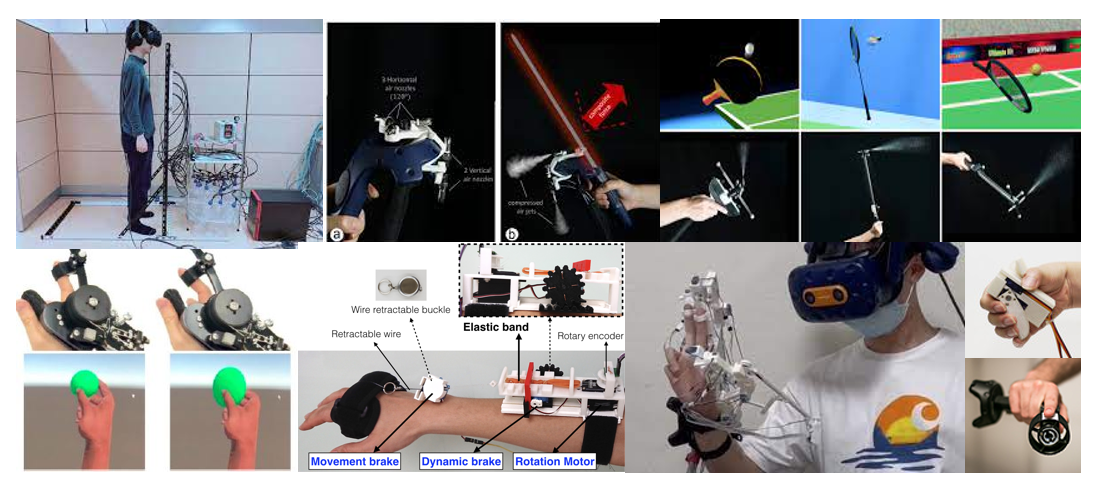
\includegraphics[width=0.75\textwidth]{A_thesis/figures/009.png}
\caption{Research cases of force group}
\end{figure}

\subsection{Innovative Interaction}
There is a category of haptic projects that can be classified according to research goals. Still, because the concepts of these studies are extremely advanced, predictive or creative, some of them cannot be simulated in real life. For example, breakthroughs that give objects interest attributes\cite{ref_EMS002}. And research on the application of haptics in mixed reality\cite{ref_EMS004}. Also the early-stage studies that focused on investigating tactile interaction between users and VR environments significantly contributed to our understanding of haptic perception\cite{ref_001}. All these researches created some more advanced human-computer interaction systems through heuristic haptic technology means. This also inspires us whether we can use new technological means to achieve new haptic experiences we did not have before, and to think about solutions that come with these new experiences.

\begin{figure}[h]
\centering
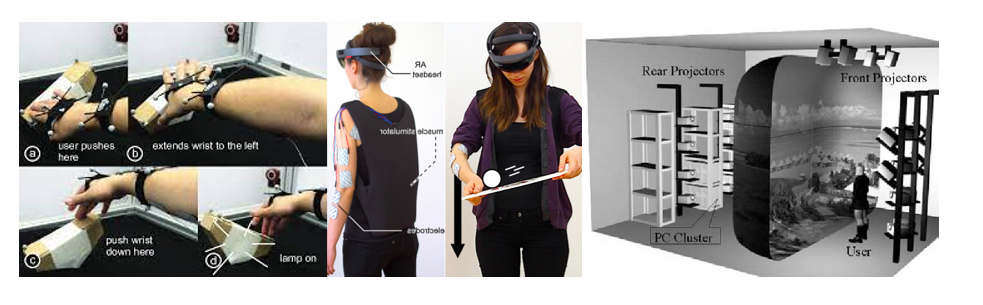
\includegraphics[width=0.75\textwidth]{A_thesis/figures/010.png}
\caption{Research cases of interaction group}
\end{figure}

\newpage

\section{Manifestation Form}
Aside from being classified by research object, device manifestation can also be divided into grounded and ungrounded.

\subsection{Grounded}
Grounded devices are physically connected to external devices or fixed to a static structure, such as the ground or a desk. Usually, grounded devices require large external devices such as air pumps\cite{ref_007}\cite{ref_008}\cite{ref_015}, power supply for driving servos, or base stations required for space trackers\cite{ref_001}. The implementation principles of these devices often involve using robotic arms or similar mechanical structures\cite{ref_010}.

\subsection{Ungrounded}
Conversely, devices that are not connected to external devices are known as ungrounded, and this is the main direction of current research. Compared to grounded devices, ungrounded devices focus more on the manifestation of specific details in virtual space. These devices usually use principles and components such as electronic vibrator\cite{ref_021} or small motors\cite{ref_018}, which require low power inputs, or devices that achieve their purpose through pseudo haptics\cite{ref_S003}. Based on more specific usage, ungrounded devices can be further divided into handheld devices, controller devices, and wearable devices.

Handheld devices refer to those that the user can directly experience with their hand. Handheld devices can be independent devices\cite{paper29}. Some haptic devices are designed to interact with smartphones by attaching to the back of the phone\cite{paper30}.

Controller devices are capable of inputting information while outputting. Common scenarios include adding pneumatic components\cite{ref_007} to existing controls, or embedding sensors in the device itself to provide haptic input such as the degree of grasping force\cite{ref_004}, rather than just joystick or button input.

In addition to these, there are quite a few wearable haptic devices, such as devices that utilize rubber bands on the arm\cite{ref_005} or research that leverages Electrical Muscle Stimulation (EMS) technology\cite{ref_EMS001}\cite{ref_EMS003}. For instance, there are devices\cite{paper31} focused on user wrist movement and force feedback. Such systems can also limit the range of user arm movements while providing haptic feedback.

With the current market development trends, including the heated discussion on the concept of haptic gloves, haptic gloves are also expected to become a new research trend.

\section{Self-motion}
In the mentioned above, we have reviewed many different types of haptic devices. There also have been some studies focused on exploring motion perception. For instance, a fixed mechanical device was used to deliver a force vector to the user's hand and wrist that aligns with the vector direction in virtual space\cite{ref_motion001}. This proved that when force feedback is provided, the user perceives motion information more clearly than when no force feedback is provided. This type of feedback can effectively enhance the user's realistic experience in a virtual environment. However, this project used large grounded haptic devices available on the market. The goal of this research is mainly focused on miniaturization, and on devices that users can use anytime. The study mentioned above demonstrated displacement in a tilt design, which is significantly different from the roller design in this research.

\begin{figure}[h]
\centering
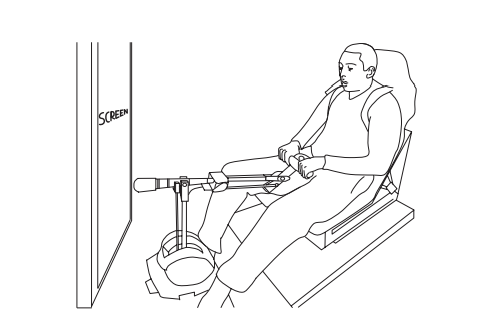
\includegraphics[width=0.6\textwidth]{A_thesis/figures/005.png}
\caption{Experimental apparatus}
\end{figure}


\newpage
Similar research\cite{ref_motion002} has explored whether providing haptic feedback on the rotation vector under passive vision scenarios and only providing visual feedback scenarios would affect the user's judgment of the rotation vector, and whether this impact is positive. In other words, the user's description of the rotation vector under haptic feedback will be more precise than under visual feedback. This is because haptic feedback can help users complete parts of the memory trajectory that did not acquire information. Although the integration of information increases the processing time for users, it enhances accuracy and completeness.

\begin{figure}[h]
\centering
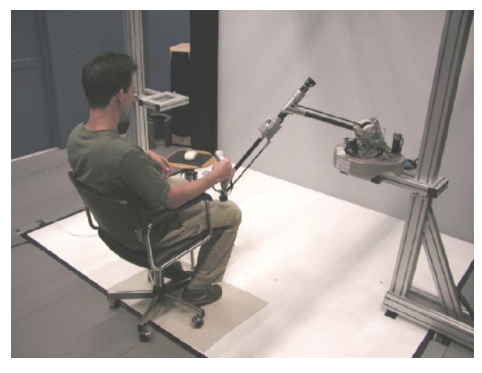
\includegraphics[width=0.5\textwidth]{A_thesis/figures/006.png}
\caption{Experimental apparatus 2}
\end{figure}

\newpage
In addition to the two studies mentioned above, some have designed and produced haptic devices for displaying motion states. For example, one study\cite{ref_motion003} placed a 6dof movable mechanical device at the user's neck and the left and right hands, simulating the user's motion information in a virtual space from the first-person perspective, including linear speed and rotational speed. However, this haptic solution may cause conflict between the vestibular sense information provided by the neck device and the visual information, resulting in simulator sickness. Therefore, another study\cite{ref_motion004} used a rotation vector to express the direction vector of forward or backward, which can effectively reduce simulator sickness.

Some researchers have considered more flexible and multi-purpose design methods. For example, a 6dof freely moving mechanical arm was linked to the manipulated controller\cite{ref_motion005}. Physical pushing and pulling forces such as dragging by the mechanical arm were used to simulate the force situation in the application. This study proved that compared with only using vision, users can more clearly feel their own sense of motion under this method.

\section{AI driving}
Because the application scenario of this research will be designed to simulate the driving environment, after verifying the effectiveness of this design, we will also conduct exploratory experiments and explorations on potential future impacts. This includes whether feeling the vehicle's motion state can enhance the user's sense of connection with the vehicle. For example, in an autonomous driving environment, the transparency of system operation and the responsibility of action consequences may affect the entire autonomous driving interaction system\cite{paper32}, and whether users can trust the autonomous driving system. 

Moreover, with the integration of automated driving systems, how new interaction interfaces and interaction methods develop will greatly influence user trust. For example, the LPD interface\cite{paper33} provided a creative design idea, projecting virtual icons onto the windshield. Another study designed\cite{paper34} a situational awareness system used to detect and adjust the current action mode in real time under autonomous driving environments. Although there is no input/output function for the vehicle's own motion information in the haptic solution, the study\cite{paper35} discussed a haptic design method for adjusting vehicle control in an autonomous driving environment.

\begin{figure}[h]
\centering
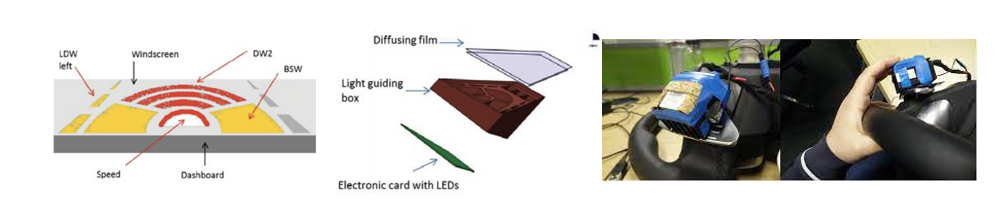
\includegraphics[width=0.8\textwidth]{A_thesis/figures/011.png}
\caption{AI driving related interaction design}
\end{figure}


\section{Summary}
By reviewing the haptics-related papers and articles, we find that most focus on static objects or common mechanical phenomena such as resistance, impact force, collision force, etc. The design preference and implementation methods are mostly ungrounded forms to facilitate user usage, better conform to close the real-world performances, provide more detailed and specific mechanical rendering, and most importantly, allow flexible usage and organic integration with virtual reality technology. For the research topic of this study, although there is no exact solution and topic for displaying the motion state of a self-moving object, many researchers have considered similar topics from different perspectives and aspects.